\clearpage
\section{Procesevaluering}
%Processen   og   gruppens   refleksion   over   processen: Læringsprocessen,  teamroller,  samarbejdet  internt  i gruppen  og  med  vejleder,  projektarbejdsformen,  arbejdsformer, metoder, skriveprocessen, den tidsmæssige styring af projektet,ledelse af projektet, arbejdsfordeling i projektet m.m. Hvordan ville I gribe arbejdet an, hvis I skulle starte forfra?
Den overordnede proces for arbejdet er forløbet relativt uproblematisk, og har fulgt en lineær model for hvordan håndteringen af projektet skulle foregå. Figuren ses på figur \ref{fig:processen} og beskriver fra start til slut, hvilke faser gruppen skal igennem, for at ende op med et færdigt projekt. Gennem processen byggede vi også vores arbejde på idéerne ved "Unified Process" og "SCRUM", som skulle sikre, at gruppen arbejdede så effektivt med projektet som muligt.\\\\
Ved projektstarts-fasen begyndte vi i gruppen, at gøre os en idé om, hvordan vi vil arbejde med casen, og samtdigt fik vi alle lavet en analyse på vores tidligere projektarbejde, med henblik på at klargøre hvilke af Belbins team-roller gruppens medlemmer passer ind på. idéen ved at starte med at give hindanden roller, hjalp til at vi kunne uddelegere opgaver mere målrette, når man internt vidste hvilke styrker hvert medlem i gruppen besidder. Vi kunne ud fra vores nyerhvervede viden om hinandens styrker og svagheder, korrigerer hvem der så fik lov at arbejde med hvad, for at sikre at de forskellige opgaver ikke ville tage for lang tid. 
\begin{figure}[H]
    \centering
    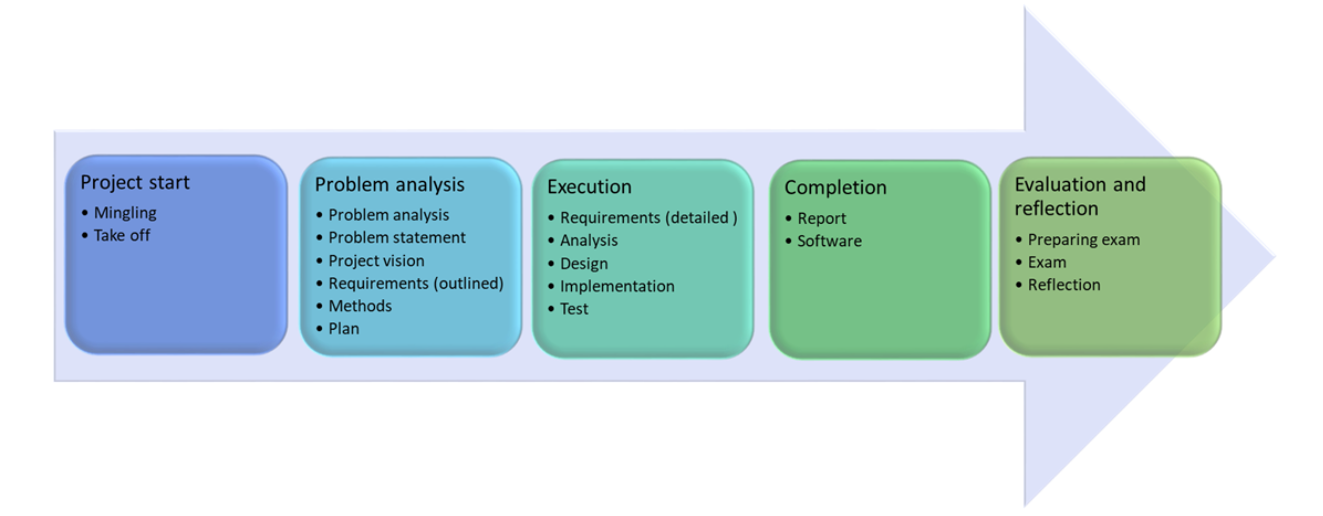
\includegraphics[width=1\textwidth]{images/processen.png}
    \caption{Processen for arbejdet med projektet}
    \label{fig:processen}
\end{figure}
Efter vores 